\begin{tabular}{c}
	
	\begin{tabular}{ | c   p{18cm} |}
		\hline
		%\rowcolor{blue!30}
		\cellcolor{black}\rotcell{\large\textbf{\textcolor{white}{Konstanten}}}  &
		\setlength{\extrarowheight}{5pt}			
		\begin{tabular}{L{5cm} L{8cm} L{3.8cm}}
			\textbf{Elektrische Feldkonstante}
			Permittivität von Vakuum &$\varepsilon_{0}=8.854 \times 10^{-12} \mathrm{~F} / \mathrm{m} $&$\left[\varepsilon_{0}\right]=\frac{\mathrm{F}}{\mathrm{m}}=\frac{\mathrm{As}}{\mathrm{Vm}}=\frac{\mathrm{C}^{2}}{\mathrm{Nm}^{2}}$\\[5pt]
			
			
			\rowcolor[rgb]{0.91,0.91,0.91}
			\textbf{Lichtgeschwindigkeit} &$\displaystyle c_0=2.99792 \times 10^{8} \mathrm{m}/\mathrm{s}=\frac{1}{\sqrt{\varepsilon_{0} \mu_{0}}}=\frac{E_{0}}{B_{0}} $
			&$\left[c_{0}\right]=\frac{\mathrm{m}}{\mathrm{s}}$\\[5pt]
			
			
			\rowcolor[rgb]{1,1,1}\textbf{Magnetische Feldkonstante}
			Permeabilität von Vakuum 
			&$\mu_{0}=4 \pi \times 10^{-7} \mathrm{H} / \mathrm{m} $&$\left[\mu_{0}\right]=\frac{\mathrm{H}}{\mathrm{m}}=\frac{\mathrm{V} \mathrm{s}}{\mathrm{A} \mathrm{m}}=\frac{\mathrm{Tm}}{\mathrm{A}}$\\[10pt]
			
			\rowcolor[rgb]{0.91,0.91,0.91}
			\textbf{Masse des Elektrons} (Ruhemasse, $v<<c_0$)
			&$m_{e}=9.109 \times 10^{-31} \mathrm{~kg} $&$\left[m_{e}\right]=\mathrm{kg}$\\[5pt]
			
			
			\rowcolor[rgb]{1,1,1}\textbf{Elementarladung}
			(Ladung des Elektrons $q_e = -e$)
			&$e=1.602 \times 10^{-19} \mathrm{C} $&$[e]=\mathrm{As}=\mathrm{C}$\\[5pt]
			
		\end{tabular}\\
		\hline
	\end{tabular}\\
\begin{tabular}{ | c   p{18cm} |}
	\hline
	\cellcolor{black}\rotcell{\large\textbf{\textcolor{white}{Geometrie}}}  &
	\begin{tabular}{p{18cm}}	
		\setlength{\extrarowheight}{10pt}			
		\begin{tabular}{L{5.6cm}| L{5.6cm}| L{5.8cm}}
			\multirow{2}{*}{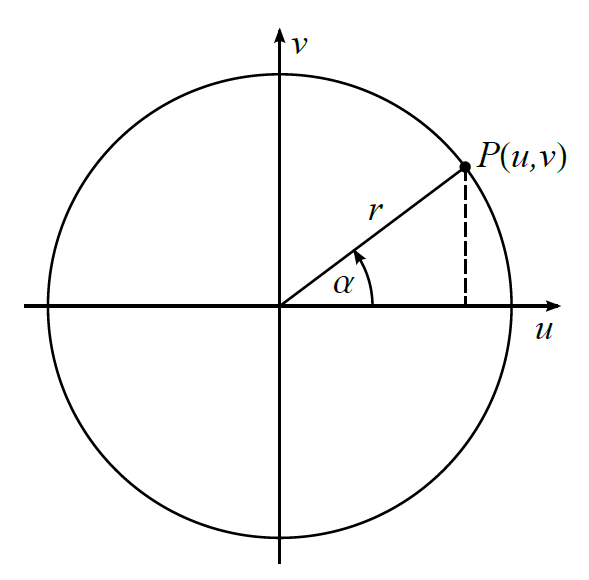
\includegraphics[width=5.6cm]{kreis.png}}
			& $\displaystyle \sin(\alpha)=\frac{v}{r}$ \qquad  $\displaystyle\cos(\alpha)=\frac{u}{r}$ &  $\displaystyle\sin(\alpha)^2  + \cos(\alpha)^2=1$\\
			&  $\displaystyle \tan(\alpha)=\frac{\sin(\alpha)}{\cos(\alpha)}$&$\displaystyle \cot(\alpha)=\frac{\cos(\alpha)}{\sin(\alpha)}$\\
			
			&$\displaystyle \sin(\alpha)=\sin(\alpha+ 2\pi)$ & $\cos(\alpha)= \cos( 2\pi-\alpha)$\\
			
			&$\displaystyle -\sin(\alpha)=\sin(-\alpha)$ & $\cos(-\alpha)= \cos(\alpha)$\\
			
			&$\displaystyle \tan(\alpha)=\tan(\alpha+ \pi)$ & $\tan(-\alpha)= -\tan(\alpha)$\\
			
			&$\displaystyle \sin(\alpha\pm\beta)=\sin(\alpha)\cos(\beta)\pm\cos(\alpha)\sin(\beta)$ & $\sin(2\alpha)= 2\sin(\alpha)\cos(\alpha)$\\
			
			&$\displaystyle \cos(\alpha\pm\beta)=\cos(\alpha)\cos(\beta)\mp\sin(\alpha)\sin(\beta)$ & $\cos(2\alpha)= \cos^2(\alpha)-\sin^2(\alpha)$\\
			
			&$\displaystyle \cos(\arcsin(x))=\sin(\arccos(x))= \sqrt{1-x^2}$ & $\cos(2\alpha)= 2\cos^2(\alpha)-1$\\
			
			
			\textbf{Kartesische Koordinaten}& \textbf{Zylindrische Koordinaten} & \textbf{Sphärische Koordinaten}\\
			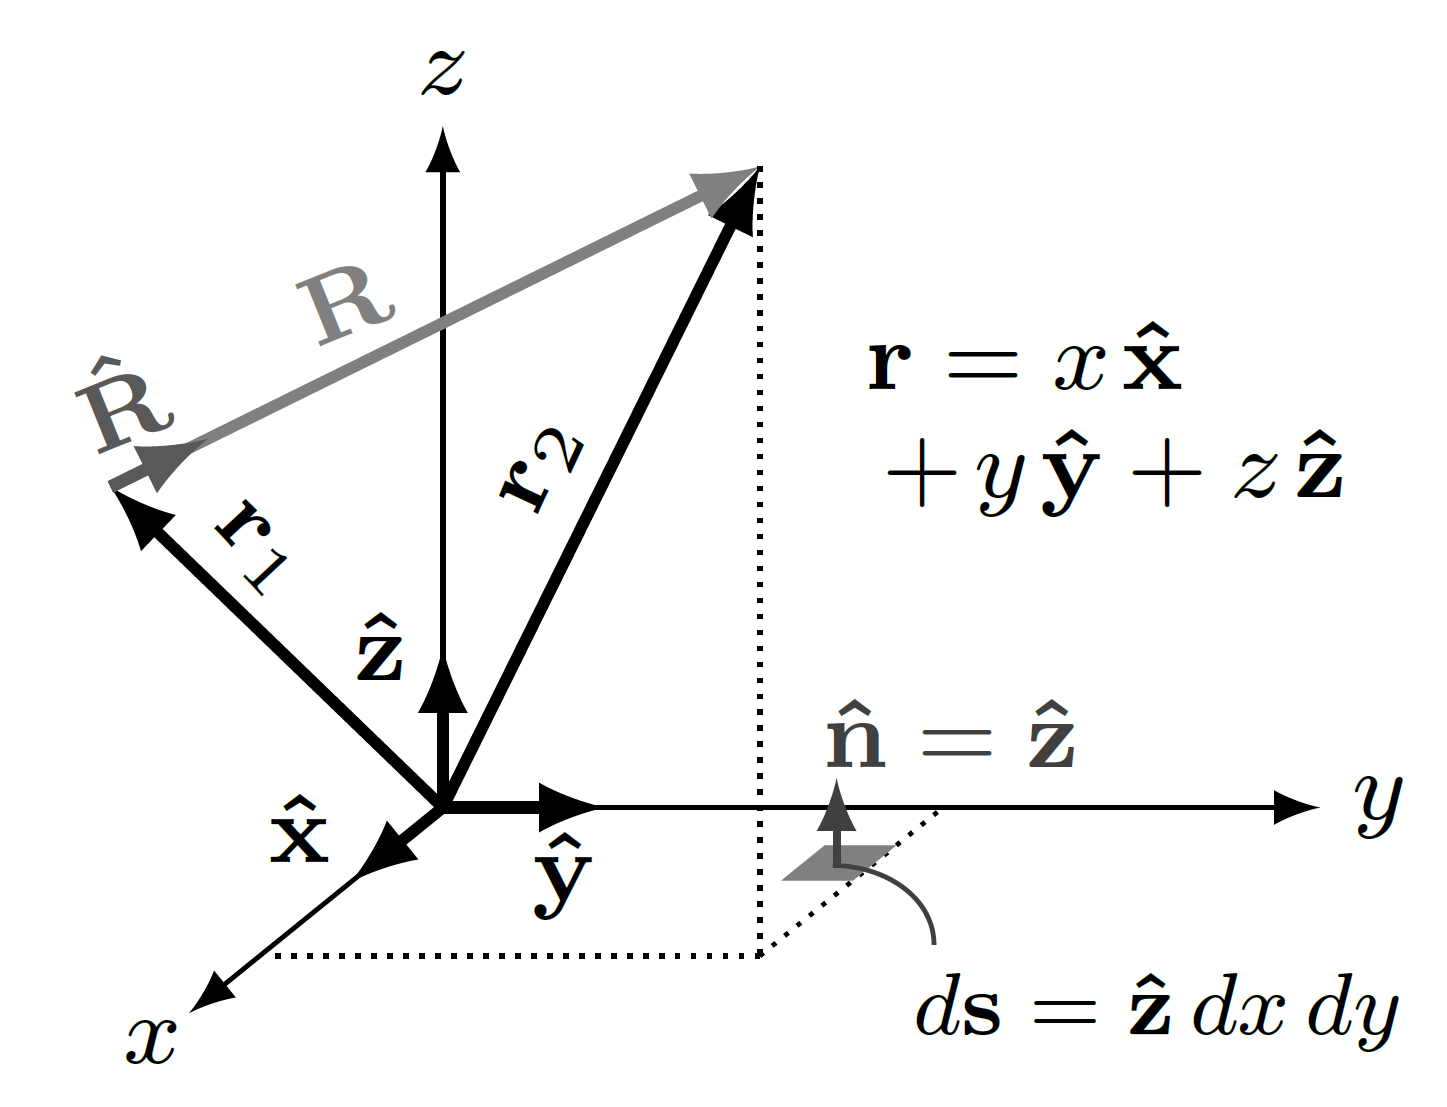
\includegraphics[width=5.6cm]{kartesische.png}& 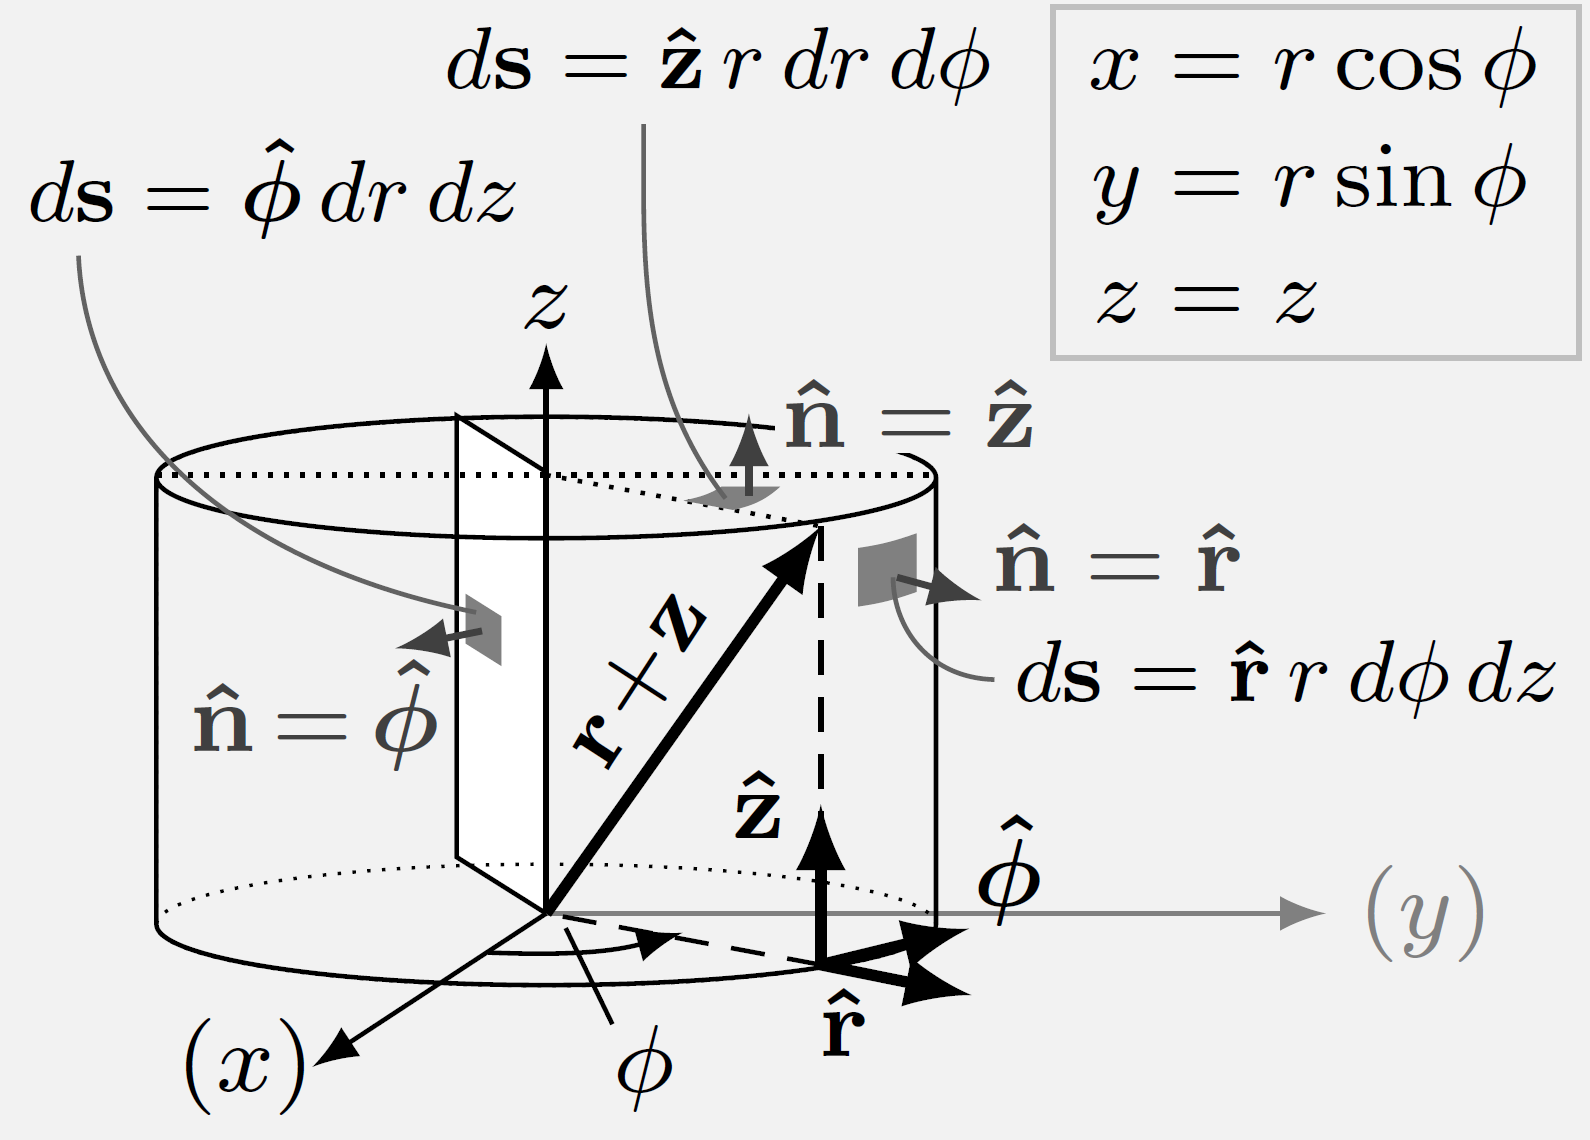
\includegraphics[width=5.6cm]{zylindrische.png}& 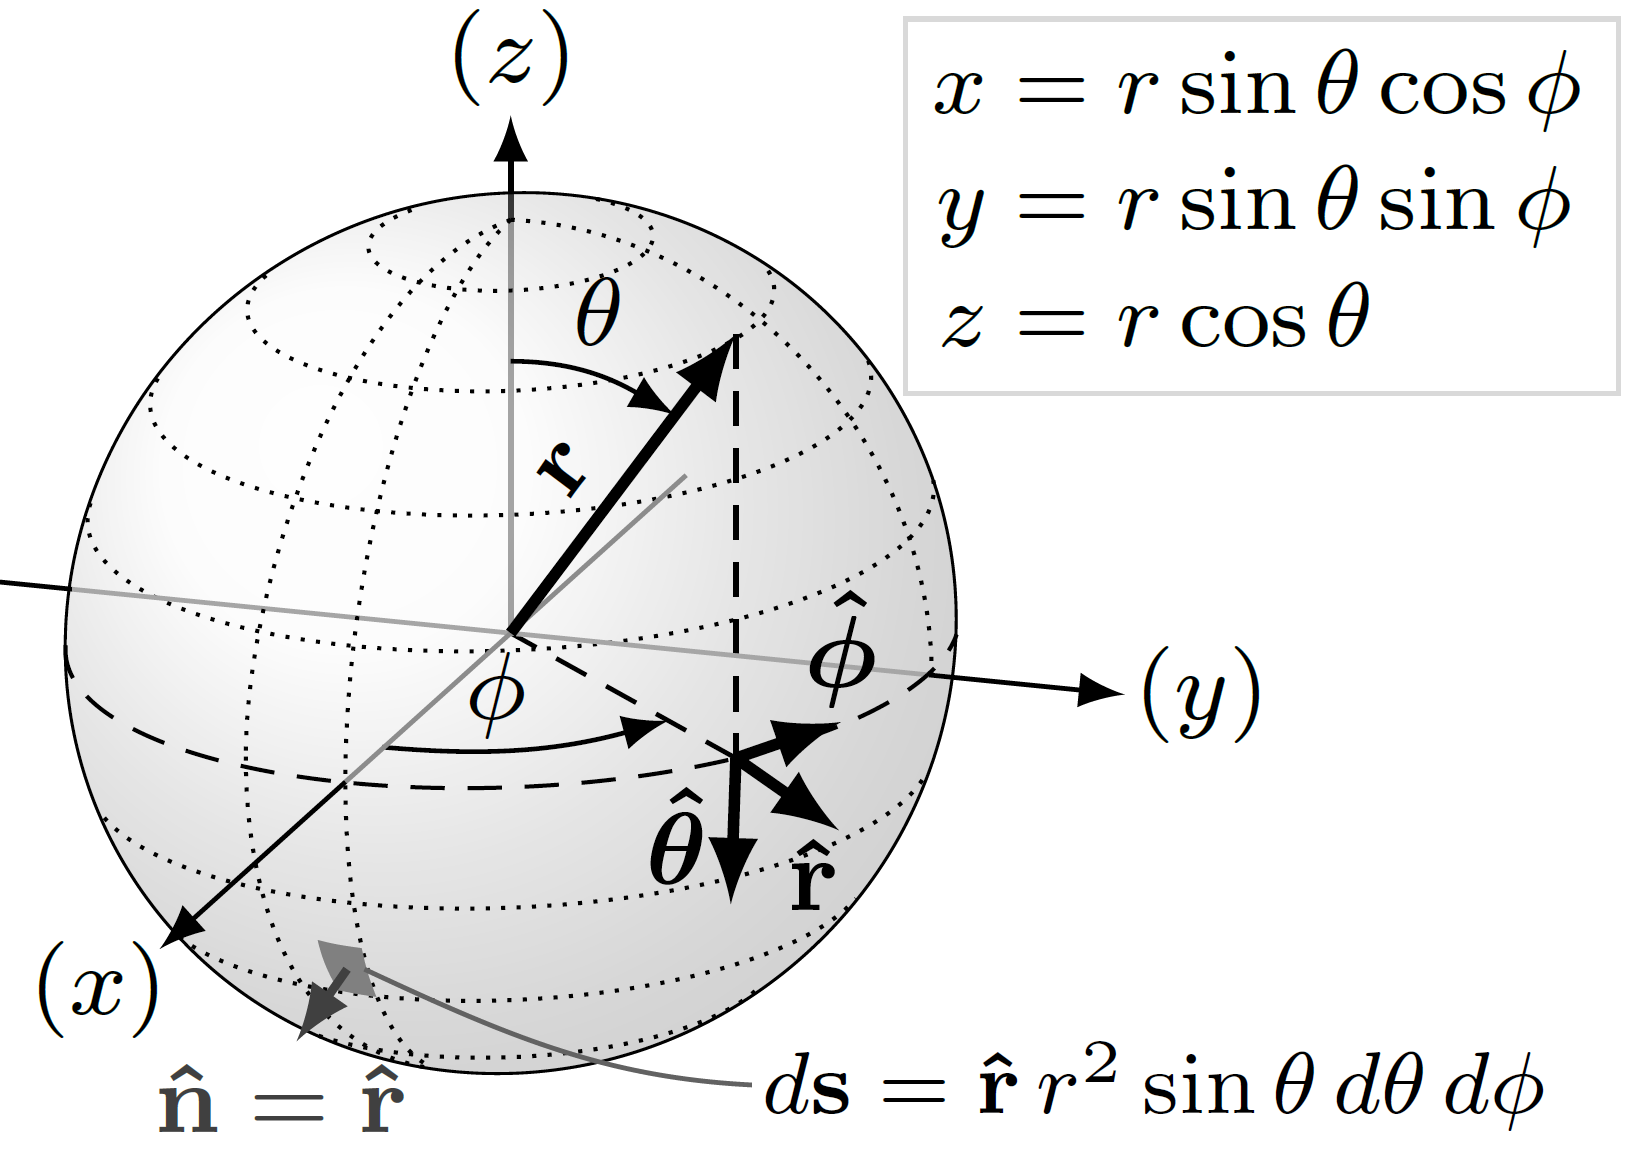
\includegraphics[width=5.6cm]{spherische.png}\\
			Volumenelement: $ d v=d x d y d z$&Volumenelement: $d v = r d r d \phi d z$&Volumenelement: $d v=r^{2} \sin \theta d r d \theta d \phi$\\
			\textbf{Kreis} Umfang $U=2\pi r$&\textbf{Oberfläche} $A=2\pi rh+2\pi r^2$ & \textbf{Oberfläche} $A=4\pi r^2$ \\
			\textbf{Kreis} Fläche $U=2\pi r^2$&\textbf{Volumen} $V=\pi r^2h$ & \textbf{Volumen} $V=\frac{4}{3}\pi r^3$ \\
			
			
			
		\end{tabular}\\
		%\setlength{\extrarowheight}{5pt}
		\begin{tabular}{L{5cm} L{7.8cm} L{3.8cm}}
			\rowcolor[rgb]{0.91,0.91,0.91}\textbf{Vektorprodukt}  $\mathbb{R}^3 \times \mathbb{R}^3 \rightarrow \mathbb{R}^3$&
			$\left(\begin{array}{c}a_{x} \\ a_{y} \\ a_{z}\end{array}\right) \times\left(\begin{array}{l}b_{x} \\ b_{y} \\ b_{z}\end{array}\right)=\left(\begin{array}{c}a_{y} b_{z}-a_{z} b_{y} \\ a_{z} b_{x}-a_{x} b_{z} \\ a_{x} b_{y}-a_{y} b_{x}\end{array}\right) $&
			$ \vec{a} \times \vec{b}=-(\vec{b} \times \vec{a})$	 \\[10pt]
			
			\rowcolor[rgb]{1,1,1}\textbf{Skalarprodukt}  $\mathbb{R}^3 \times \mathbb{R}^3 \rightarrow \mathbb{R}$&
			$\left(\begin{array}{l}a_{x} \\ a_{y} \\ a_{z}\end{array}\right) \cdot\left(\begin{array}{l}b_{x} \\ b_{y} \\ b_{z}\end{array}\right)=a_{x} b_{x}+a_{y} b_{y}+a_{z} b_{z}=\vec{a} \cdot \vec{b} $&
			$\displaystyle \cos (\varphi)=\frac{\vec{a} \cdot \vec{b}}{|\vec{a}| \cdot|\vec{b}|}$\\[5pt]
			
			\rowcolor[rgb]{0.91,0.91,0.91}
			\textbf{Komplexe Polarform}
			&$\displaystyle z = r\cdot e^{i\varphi} = r\cos(\varphi)+i\sin(\varphi)$
			&$\displaystyle z = a +bi$\qquad $r= |z|= \sqrt{a^2 +b^2}$ \\[5pt]
			
			\rowcolor[rgb]{1,1,1}
			\textbf {Komplexe Winkel} &$\displaystyle \varphi= \arg(z)= \begin{cases}\displaystyle \arccos(\frac{a}{r})  \\ \displaystyle -\arccos(\frac{a}{r} ) \end{cases} $&
			$\displaystyle \begin{cases} b\geq0 \\ \displaystyle b<0 \end{cases}$\\[5pt]
			
			\rowcolor[rgb]{0.91,0.91,0.91}\textbf{Arithmetik}&
			$z_1 = r_1 cis(\varphi_1)= r_1e^{i\varphi_1}$&
			$z_2 = r_2 cis(\varphi_2)= r_2e^{i\varphi_2}$		\\
			
			\textbf{Winkel Addieren}&$z_1\cdot z_2 = r_1\cdot r_2 \text{cis}(\varphi_1+\varphi_2)$&	\\
			
			\textbf{Winkel Subtrahieren}&$z_1/ z_2 = r_1/r_2 cis(\varphi_1-\varphi_2)$&	\\[5pt]
			
			
			
			
			
		\end{tabular}\\[5pt]
	\end{tabular}\\
	\hline	
\end{tabular}

	
\end{tabular}
	